% NICOLE CAMILLE BAIÃO - PRAXISTRANSFERBERICHT II

% === DOKUMENTKLASSE ===
\documentclass[
    12pt, 
    a4paper,
    ]{scrartcl} % KOMA-Script-Artikelklasse mit deutscher Typografie

% === SPRACHE & ZEICHENSATZ ===
\usepackage[ngerman]{babel} % Deutsche Sprache und Silbentrennung
\usepackage{csquotes} % Typografisch korrekte Anführungszeichen

% === SEITENLAYOUT & FORMATIERUNG ===
\usepackage[a4paper, margin=2.5cm]{geometry}
\usepackage{setspace}
\setstretch{1.15}
\usepackage{fancyhdr}
\usepackage{float} % Exakte Platzierung von Gleitobjekten (z. B. Bilder)
\usepackage{caption} % Bild-/Tabellenbeschriftungen anpassen
\usepackage{adjustbox} % Elemente (z. B. Tabellen) skalieren oder ausrichten
\usepackage{makecell} % Mehrzeilige Zellen in Tabellen (Tabellen in Tabellen)
\usepackage{ragged2e}
\justifying 
% === SCHRIFTARTEN ===
\usepackage{iftex} % Prüft, ob XeTeX oder LuaTeX verwendet wird
\usepackage{fontspec} % Benutzerdefinierte Schriftarten (nur mit XeLaTeX/LuaLaTeX)
\usepackage{titlesec}
% Aktuelle Größen beibehalten:
\titleformat{\section}{\normalfont\fontsize{14}{5}\bfseries}{\thesection}{1em}{}
\titleformat{\subsection}{\normalfont\fontsize{13}{5}\bfseries}{\thesubsection}{1em}{}
\titleformat{\subsubsection}{\normalfont\fontsize{12}{5}\bfseries}{\thesubsubsection}{1em}{} 

% ABSTÄNDE ANPASSEN — Das ist der Schlüssel:
\titlespacing*{\section}{0pt}{1.1\baselineskip}{0.1\baselineskip}
\titlespacing*{\subsection}{0pt}{1.0\baselineskip}{0.1\baselineskip}
\titlespacing*{\subsubsection}{0pt}{0.9\baselineskip}{0.1\baselineskip}
 % Hauptschriftart
\setmainfont{Times New Roman} % Setzt Times New Roman als Hauptschrift

% === GRAFIKEN & ABBILDUNGEN ===
\usepackage{graphicx} % Bilder einfügen
\usepackage{xcolor} % Farben verwenden (z. B. in Code oder Text)
\usepackage{longtable}
\usepackage{tablefootnote}
% === QUELLEN & VERWEISE ===
\usepackage{cite} % Quellenangaben
\usepackage[
    colorlinks,       % Links ohne Umrandungen in gewählter Farbe
    linkcolor=black,  % Farbe interner Verweise
    filecolor=black,  % Farbe externer Verweise
    citecolor=black,  % Farbe von Zitaten
    urlcolor=black,    % Farbe von Links
    breaklinks
]{hyperref} % Verlinkungen
\usepackage{cleveref} % Querverweise der Querverweise
\newcommand{\etalchar}[1]{#1}

% === TABELLEN ===
\usepackage{longtable} % Tabellen über mehrere Seiten
% makecell wurde oben bereits geladen

% === CODE-DARSTELLUNG ===
\usepackage{listings} % Quellcode einfügen und formatieren

%%%%%%%%%%%%%%%%%%%%%%%%%%

% === ÜBERSCHRIFTEN-FORMATIERUNG ===
\setkomafont{sectioning}{\rmfamily\bfseries} % Überschriften fett und serifenlos

% === VERLINKUNGEN & REFERENZEN ===
\hypersetup{breaklinks=true} % Erlaubt Zeilenumbruch bei langen Links (wichtig für URLs oder Literaturverweise)
\newcommand{\anhang}[1]{\hyperref[#1]{\nameref{#1}}} % Eigener Befehl für Anhang-Verweise mit automatisch lesbarem Namen (anstatt z. B. nur "Abschnitt 5.1")

% === SEITENLAYOUT & RÄNDER ===
\geometry{
    verbose,
    tmargin=3cm,  % Oberer Rand
    bmargin=2cm,  % Unterer Rand
    lmargin=2.1cm,  % Linker Rand
    rmargin=3cm   % Rechter Rand
}

% === TYPOGRAFISCHE FEINHEITEN ===
\displaywidowpenalty = 5000
\widowpenalty=5000
\clubpenalty=5000
% === FUßNOTEN UND VERWEISE ===
\newcommand{\footfigref}[1]{\footnote{Abb. \ref{#1} auf Seite \pageref{#1}}} % Eigener Fußnotenbefehl für Bildverweise mit Seitenzahl

% === ABSTÄNDE & ABSATZFORMATIERUNG ===
\setlength{\footskip}{10mm} % Abstand zwischen Text und Fußzeile
\setlength{\abovecaptionskip}{4pt}  % Abstand oberhalb von Bild-/Tabellenunterschriften
\setlength{\belowcaptionskip}{0pt}  % Abstand unterhalb von Bild-/Tabellenunterschriften
\setlength{\intextsep}{1pc}         % Abstand bei Gleitobjekten (z. B. Bilder im Textfluss)
\setlength{\parindent}{0pt} % Kein Einzug am Absatzanfang
\setlength{\parskip}{0.75\baselineskip} % Einheitlicher Abstand zwischen Absätzen
\setstretch{1.5} % 1½-zeiliger Zeilenabstand
% === BILD- UND TABELLENUNTERSCHRIFTEN VERKLEINERN ===
\addtokomafont{caption}{\small} % Macht Bild-/Tabellenunterschriften kleiner

% === INHALTSVERZEICHNIS & LISTEN ===
\KOMAoptions{listof=entryprefix, toc=indent} % Inhaltsverzeichnis: eingerückt und mit Präfix bei Abbildungs-/Tabellenlisten

% === CODEDARSTELLUNG (SQL) ===
\lstdefinelanguage{SQL}{
    keywords={SELECT, FROM, WHERE, INSERT, INTO, VALUES, UPDATE, SET, DELETE, JOIN, LEFT, RIGHT, INNER, ORDER, BY, GROUP, ASC, DESC, CREATE, TABLE, PRIMARY, KEY, FOREIGN, ALTER, DROP, DATABASE, BEGIN, TRANSACTION, IF, EXISTS, COMMIT, AND},
    keywordstyle=\color{blue},           % Keywords blau
    comment=[l]{--},                     % Kommentare mit --
    morecomment=[s]{/*}{*/},             % Blockkommentare
    commentstyle=\color{gray},          % Kommentare grau
    stringstyle=\color{red},            % Strings rot
}

\lstset{
    basicstyle=\ttfamily\linespread{0.85}\selectfont,   % Standard-Monospace-Schrift für Listings
    keywordstyle=\bfseries\color{blue},  % Beispiel-Stil für Keywords
    commentstyle=\itshape\color{gray},   % Stil für Kommentare
    stringstyle=\color{red},            % Stil für Strings
    columns=flexible,       % Flexibler Zeilenumbruch
    language=SQL,
    breaklines=true
}

%%%%%%%%%%%%%%%%%%%%%%%%%%

% === BEGINN DOKUMENT ===
\begin{document}
% === LITERATUR EINBINDEN (unsichtbar zitieren, damit sie im Literaturverzeichnis auftaucht) ===

% --- Seitenzahlen-Formatierung 1/3: Römische Zahlen ---
\pagenumbering{Roman}  % Nutzt römische Zahlen (I, II, III, …)
\pagestyle{fancy}      % Aktiviert fancyhdr für benutzerdefinierte Kopf-/Fußzeilen
\fancyhf{}             % Setzt alle Kopf- und Fußzeilen zurück
\fancyhead[R]{\thepage}  % Seitenzahl oben rechts anzeigen
\renewcommand{\headrulewidth}{0pt} % Keine Linie in der Kopfzeile
\renewcommand{\footrulewidth}{0pt} % Keine Linie in der Fußzeile

%%%%%%%%%%%%%%%%%%%%%%%%%%

% === BEGINN TITELSEITE ===
\begin{titlepage}
\centering % Zentriert den gesamten Inhalt der Titelseite
   
% --- Logos einfügen (links und rechts) ---

\includegraphics[scale=0.15]{BILDER-PTB2/Berliner-wasserbetriebe.svg.png}\hfill % \hfill sorgt dafür, dass die beiden Logos links und rechts stehen

\includegraphics[scale=0.25]{BILDER-PTB2/Hochschule_für_Wirtschaft_und_Recht_Berlin_logo.jpg} \\[0.7cm] % \\[1.8cm] fügt einen vertikalen Abstand von 1.8 cm nach den Bildern ein

% --- Titel (fette und große Schrift) ---
\Large{\textbf{Handlungsempfehlungen für die Skalierung der Prozesse zur Einführung von Software-Produkten - am Beispiel der erweiterten Nutzung der Adobe Creative Cloud}} \\[0.3cm]
    \doublespacing % Verdoppelt den Zeilenabstand

% --- Untertitel ---
{\Large Praxistransferbericht II} \\
\singlespacing % Setzt den Zeilenabstand wieder auf normalen Wert

% --- Neuer Text mit Abstand --
\vspace{0.1cm} % Abstand zum Unterschift
\large % Setzt die Schriftgröße auf Standard
vorgelegt am 29.09.2025 an der\\ [0.2cm]
Hochschule für Wirtschaft und Recht Berlin\\ [0.2cm]
Fachbereich Duales Studium\\ [0.2cm]
\vspace{0.6cm} % Abstand zur Tabelle

% --- Tabelle mit persönlichen Angaben ---
\begin{tabular}{l l}  
    \textbf{\normalsize{von:}} & \normalsize{Nicole Camille Baião}  \\[0.2cm]
    \textbf{\normalsize{Bereich:}} & \normalsize{Wirtschaft} \\[0.2cm]
    \textbf{\normalsize{Fachrichtung:}} & \normalsize{Wirtschaftsinformatik} \\[0.2cm]
    \textbf{\normalsize{Studienjahrgang:}} & \normalsize{2024} \\[0.2cm]
    \textbf{\normalsize{Studienhalbjahr:}} & \normalsize{2. Semester} \\[0.2cm]
    \textbf{\normalsize{Ausbildungsbetrieb:}} & \normalsize{Berliner Wasserbetriebe}  \\[0.2cm]
    \textbf{\normalsize{Betreuender Prüfer:}} & \normalsize{Philip Dreßel} \\[0.2cm]
    \textbf{\normalsize{Betreuer im Betrieb:}} & \normalsize{Fenja Helbig} \\[1.25cm]
\end{tabular} 

% --- Bereich für Unterschriften ---
\raggedright % Setzt den folgenden Text linksbündig
\textbf{\normalsize{Vom Ausbildungsleiter zur Kenntnis genommen:}} \\[0.5cm]

% --- Tabelle mit Unterschriften ---
\begin{tabular}{p{8cm} p{8cm}}
    \normalsize{Berlin, den 27. September 2025} & \normalsize{Berlin, den 28. September 2025} \\[0.4cm]

    
\includegraphics[width=5.7cm]{BILDER-PTB2/unterschrift_nicole.png} &
    
\includegraphics[width=4cm]{BILDER-PTB2/unterschrift_max.png} \\[0.1cm]

    \normalsize{\underline{\hspace{5cm}}} & \normalsize{\underline{\hspace{5cm}}} \\[0.1cm]
    \normalsize{(Unterschrift der Studentin)} & \normalsize{(Unterschrift des Ausbildungsleiters)}
\end{tabular}
% === ENDE TITELSEITE ===
\end{titlepage}

% === Inhaltsverzeichnis === 
\setcounter{page}{1} % Setzt die Seitennummer auf 1 für neue Zählung (Neustart der Zählung)
\newpage
\section*{Inhaltsverzeichnis}  
\renewcommand{\contentsname}{}
\vspace{-1.3cm}  % Anpassung des vertikalen Abstands
\tableofcontents % Inhaltsverzeichnis erstellen

% === Abküzungsverzeichnis === 
\newpage
\section*{Abkürzungsverzeichnis}  
\addcontentsline{toc}{section}{Abkürzungsverzeichnis}
\vspace{0.6cm}
\begin{tabular}{p{4cm} p{11.35cm}}   
    \textbf{\normalsize BWB} & \normalsize Berliner Wasserbetriebe \\[0.5cm]
    \hline
    \textbf{\normalsize IT} & \normalsize Informationstechnologie \\[0.5cm]
    \hline
    \textbf{\normalsize ITIL} & \normalsize IT Infrastructure Library \\[0.5cm]
    \hline
    \textbf{\normalsize KI} & \normalsize Künstliche Intelligenz \\[0.5cm] 
\end{tabular}

% --- Seitenzahlen-Formatierung 2/3: Wechsel auf normale (arabische) Zahlen ---
\newpage
\pagenumbering{arabic} % Normale Zahlen ab "Einleitung"
\setcounter{page}{1}
% === Einleitung ===
\section{Einleitung}

Die Berliner Wasserbetriebe (BWB) sind das größte Wasserver- und Abwasserentsorgungsunternehmen Deutschlands und zugleich einer der größten Arbeitgeber in Berlin. Das Unternehmen beschäftigt aktuell 4.836 Mitarbeitende.\footnote{Vgl. \cite{S_BWB}.} In einem derart komplexen Umfeld mit zahlreichen Fachabteilungen und hohen regulatorischen Anforderungen übernimmt die IT-Abteilung eine zentrale Rolle.

Innerhalb der IT ist die Abteilung Kundenberatung und Anforderungsmanagement für die internen Kunden der BWB zuständig. Sie berät die Fachbereiche, nimmt deren Bedarfe auf, bewertet sie und entwickelt in Abstimmung mit den zentralen IT- und Portfoliomanagement-Einheiten passende Lösungen.\footnote{Vgl. \cite{S_Asana}.} Dies kann sowohl die Einführung neuer Anwendungen als auch die Anpassung oder Erweiterung bestehender Systeme umfassen.\footnote{Vgl. \cite{S_ISR}.} Anforderungen können dabei etwa Funktionen sein, die eine erfolgreiche Nutzung ermöglichen, oder Aspekte, die Abteilungen bei der Erreichung ihrer Geschäftsziele unterstützen.\footnote{Vgl. \cite{S_ISR}.}

Vor diesem Hintergrund gewinnt die Nutzung von Cloud-Software zunehmend an Bedeutung. Am Beispiel der Adobe Creative Cloud zeigt sich, dass moderne KI-Funktionalitäten\footnote{Vgl. \cite{S_AdobeAI}, \cite{S_AdobeCloud}.} erhebliche Chancen für Effizienzsteigerungen bieten, gleichzeitig jedoch auch Risiken mit sich bringen.\footnote{Vgl. \cite{S_Ambient}.} Besonders relevant ist die Frage, wie bestehende Softwareprodukte erweitert und skaliert werden können, sodass keine vollständige Neubeschaffung erforderlich wird.

Das Ziel dieser Arbeit ist es daher, anhand des Falls der erweiterten Nutzung der Adobe Cloud aufzuzeigen, wie Anforderungen systematisch analysiert und bewertet werden können, um daraus Handlungsempfehlungen für künftige ähnliche Szenarien abzuleiten. Hierzu werden theoretische Konzepte aus ITIL, Change- und Anforderungsmanagement mit praktischen Erfahrungen im Anforderungsprozess verknüpft. Zur Ergänzung werden Interviews mit Mitarbeitenden der Berliner Wasserbetriebe herangezogen, die praxisnahe Einblicke und Erfahrungen liefern. Die Ausarbeitung erfolgt in LaTeX.

% === Theoretischer Rahmen ===
\section{Theoretischer Rahmen}
\subsection{Software-Einführung und -Erweiterung}
In der Literatur finden sich unterschiedliche Definitionen des Begriffs Softwareeinführung. Nach einer engeren Auffassung bezeichnet er ausschließlich die erstmalige Implementierung einer neuen Anwendung in einem Unternehmen und umfasst damit vor allem die technische Installation, Inbetriebnahme und Akzeptanz durch die Mitarbeitenden.\footnote{Vgl.\cite{papershift2022}.} 
Eine erweiterte Definition geht darüber hinaus: Sie versteht Softwareeinführung nicht nur als einmalige Implementierung, sondern auch als Anpassung oder Erweiterung neuer Softwarelösungen. Jede Änderung oder neue Nutzungssituation bedeutet somit eine erneute „Einführung“ – auch wenn es sich nicht um ein komplett neues Produkt handelt.\footnote{Vgl.\cite{pureconsultant2023}.}

Für ein großes Unternehmen wie die Berliner Wasserbetriebe sind beide Definitionen relevant. Einerseits werden regelmäßig neue Anwendungen eingeführt, andererseits spielen die Anpassung und Erweiterung bestehender Softwarelösungen eine zentrale Rolle. In dieser Arbeit liegt der Fokus jedoch auf der Erweiterung und Skalierung bereits genutzter Software, wie dies am Beispiel der Adobe Cloud deutlich wird.\footnote{Vgl.\cite{softwarevergleich2023}.}
Ein strukturierter Ablauf ist entscheidend für den Erfolg. Typischerweise wird der Prozess in fünf Phasen gegliedert, die sich an Projektmanagement- und ITIL-Strukturen orientieren:
\begin{enumerate}
    \item \textbf{Projektvorbereitung} – Festlegung von Zielen, Nutzen und Projektteam.
    \item \textbf{Planung} – Ausarbeitung von Konzept, Prozessen, Ressourcen und Risiken.
    \item \textbf{Auswahl der Software} – systematische Evaluierung und Pilotierung.
    \item \textbf{Installation \& Rollout} – Umsetzung, Datenmigration, Tests und Übergabe.
    \item \textbf{Überwachung \& Analyse} – Betrieb, Support und kontinuierliche Optimierung.\footnote{Vgl.\cite{papershift2022}.} 
\end{enumerate}
Bei einer Software-Erweiterung, die im Mittelpunkt dieser Arbeit steht, sind hingegen nur einzelne Phasen in vollem Umfang relevant. Welche dies konkret sind, wird im weiteren Verlauf noch verdeutlicht.  
 \subsection{Cloud-Software und KI-Funktionalitäten}

Die zunehmende Nutzung von Cloud-Software hat die Dynamik der Einführung und Erweiterung von Anwendungen grundlegend verändert. Cloud-Lösungen sind skalierbar, ortsunabhängig verfügbar und lassen sich vergleichsweise einfach aktualisieren.\footnote{Vgl. \cite{S_BSI_Grundlagen}, S.~5.} Gleichzeitig stellen sie Unternehmen vor neue Herausforderungen, insbesondere im Hinblick auf Datensicherheit, die Einhaltung gesetzlicher Vorgaben und eine mögliche Abhängigkeit vom Anbieter.\footnote{Vgl. \cite{S_BSI_Risiken}, S.~7.}

Hinzu kommt, dass viele Cloud-Produkte heute mit KI-Funktionalitäten ausgestattet sind. Diese eröffnen Chancen wie die Automatisierung von Prozessen, die Unterstützung kreativer Tätigkeiten oder die Verbesserung der Entscheidungsqualität.\footnote{Vgl. \cite{S_BSI_KI}, S.~9.} Gleichzeitig bergen sie Risiken: der Umgang mit sensiblen Daten, die oft in externen Rechenzentren verarbeitet werden, wirft Fragen zum Datenschutz auf.\footnote{Vgl. \cite{S_ENISA_AI}, S.~24-26.} Auch die mangelnde Transparenz sogenannter „Black-Box-Algorithmen“ kann problematisch sein.\footnote{Vgl. \cite{S_ENISA_AI}, S.~9.} Unternehmen müssen daher Chancen und Risiken abwägen und geeignete Governance-Strukturen schaffen. Die spezifische Vorgehensweise der BWB wird im weiteren Verlauf praxisnah dargestellt.

\subsection{ITIL-Best Practices}

Die ITIL ist ein zentraler Bestandteil für das Verständnis von Software-Erweiterungen im IT-Service-Management. Um seine Rolle nachvollziehen zu können, ist es notwendig, zunächst einige grundlegende Begriffe zu klären. Ein IT-Service ist eine immaterielle Dienstleistung der Informationstechnologie, die unter anderem Beratung, Planung sowie die Bereitstellung von Hardware- und Softwareleistungen umfasst. ITIL definiert ihn als „ein oder mehrere IT-Systeme, die einen Geschäftsprozess ermöglichen oder unterstützen und vom Kunden als zusammenhängendes Ganzes wahrgenommen werden“.\footnote{Vgl. \cite{S_ITIL}, S.~6.} 

Die Qualität des Service spielt dabei eine zentrale Rolle und wird durch kontinuierliche Steuerung und Verbesserung gesichert. Aufbauend darauf versteht man unter IT-Service-Management (ITSM) ein prozessorientiertes Modell, das die Gesamtheit der Methoden und Prozesse zur Lieferung, Unterstützung und Steuerung von IT-Services umfasst. Ziel ist es, die IT-Infrastruktur und Anwendungen so auszurichten, dass sie die Geschäftsziele bestmöglich unterstützen.\footnote{Vgl. \cite{S_ITIL}, S.~8, S.~139.}

Als Rahmenwerk dient hier die IT Infrastructure Library (ITIL), die in den 1980er-Jahren im Auftrag der britischen Regierung entwickelt wurde.\footnote{Ebenda, S.~11--12.} Sie beruht auf dem sogenannten Best-Practice-Ansatz, also einer Vereinheitlichung der Analyseergebnisse britischer Behörden, die ihre gesammelten Erfahrungen in einer Büchersammlung dokumentierten.\footnote{Ebenda, S.~123.} ITIL legt damit fest, was und wann im IT-Service-Management zu tun ist, ohne jedoch das Wie vorzuschreiben.\footnote{Ebenda, S.~124.} 

\subsection{Rolle des Anforderungsmanagements}

Das Requirements Engineering (Anforderungsmanagement) ist ein systematischer und disziplinierter Prozess, bei dem die Bedürfnisse, Erwartungen und Anforderungen an ein System erfasst, analysiert, dokumentiert, geprüft und verwaltet werden.\footnote{Vgl. \cite{S_PohlRupp}, S.~3--4.} Solche Bedürfnisse werden im wirtschaftlichen Sinn als Bedarf bezeichnet, also ein konkretisiertes Bedürfnis, das durch eine Leistung oder Lösung erfüllt werden kann.\footnote{Vgl. \cite{S_WikipediaBedarf}.}

Im Mittelpunkt des Requirements Engineering steht der Begriff des Stakeholders. Als Stakeholder gelten alle Personen oder Organisationen, die in irgendeiner Weise Einfluss auf die Anforderungen eines Systems haben. Dazu zählen etwa spätere Nutzer, Administratoren, das Management oder auch externe Institutionen. Wichtig ist: Anforderungen entstehen nicht isoliert, sondern immer im Kontext der Interessen und Bedürfnisse dieser Stakeholder.\footnote{Vgl. \cite{S_PohlRupp}, S.~3--4.}

Ziel des Requirements Engineering ist es, sicherzustellen, dass alle relevanten Anforderungen korrekt verstanden und über den gesamten Projektverlauf hinweg berücksichtigt werden. Ein zentrales Element dabei ist die Fähigkeit, flexibel auf veränderte Rahmenbedingungen und neue Anforderungen zu reagieren. Requirements Engineering ist also kein einmaliger Schritt, sondern ein kontinuierlicher Prozess der Anpassung und Weiterentwicklung.\footnote{Vgl. \cite{S_ISR}.} 

Um diese Anforderungen erfolgreich umzusetzen, gliedert sich das Requirements Engineering in folgende zentrale Tätigkeiten: Ermitteln, Dokumentieren, Prüfen und Abstimmen sowie Verwalten. Beim Ermitteln geht es darum, mithilfe geeigneter Methoden (z. B. Interviews, Beobachtungen) die relevanten Anforderungen der Stakeholder zu identifizieren. In der Phase des Dokumentierens werden diese systematisch festgehalten. Danach folgt das Prüfen und Abstimmen, bei dem Anforderungen mit Stakeholdern abgeglichen und auf Konsistenz, Vollständigkeit und Verständlichkeit überprüft werden. Abschließend sorgt das Verwalten dafür, dass Anforderungen über den Projektverlauf hinweg aktuell bleiben und bei Änderungen angepasst werden.\footnote{Vgl. \cite{S_PohlRupp},S.~4--5.}

\subsection{Change Management}

Change Management bezeichnet die bewusste und strukturierte Steuerung von Veränderungsprozessen in Organisationen. Ziel ist es, Veränderungen gezielt einzuleiten, zu steuern und nachhaltig abzusichern.\footnote{Vgl. \cite{S_Schichtel}, S.~40.} Dabei reicht es nicht, technische Anpassungen vorzunehmen – im Mittelpunkt steht die aktive Einbindung der betroffenen Menschen, da jede Veränderung ihre bestehenden Denk- und Verhaltensmuster sowie Arbeitsabläufe beeinflusst.

Ein wesentliches Merkmal des Change Managements besteht darin, dass die emotionale Ebene der Betroffenen berücksichtigt, Orientierung geschaffen und ein gemeinsames Vorgehen ermöglicht wird.\footnote{Ebenda, S.~41.} Damit Veränderungen akzeptiert und erfolgreich umgesetzt werden können, spielen drei Ebenen eine zentrale Rolle: Strategie (Zielrichtung und Vision), Struktur (Prozesse und organisatorische Abläufe) sowie Kultur (Werte, Einstellungen und Verhaltensweisen).\footnote{Ebenda, S.~43.} Diese Ebenen greifen ineinander und entscheiden darüber, ob ein Veränderungsprozess im Alltag verankert wird.
Transparente Kommunikation ist dafür entscheidend: Nur wenn Ziele, Hintergründe und Auswirkungen klar vermittelt werden, entsteht Akzeptanz und Beteiligung. Besonders bei Softwareanpassungen zeigt sich, dass Change Management nicht allein technische Maßnahmen umfasst, sondern immer auch den sozialen Kontext und die Bedürfnisse der Beteiligten.\footnote{Ebenda, S.~42--43.}

% === 3. Praxisteil ===
\section{Anforderungsmanagement in der Praxis}

Die Berliner Wasserbetriebe nutzen seit vielen Jahren Adobe-Produkte in der Unternehmenskommunikation, bisher in Form der lokal installierten Creative Suite. Da dieses Produkt von Adobe eingestellt wurde, erfolgte der notwendige Umstieg auf die cloudbasierte Adobe Creative Cloud. Um die Arbeitsfähigkeit sofort zu sichern, wurden zunächst nur die bereits bekannten Werkzeuge freigeschaltet – ohne neue Cloud- oder KI-Funktionen.

\subsection{Bedarfsaufnahme}

Parallel äußerte die Unternehmenskommunikation den Wunsch nach einem erweiterten Zugriff auf zusätzliche Komponenten, insbesondere auf die in der Creative Cloud integrierten KI-gestützten Funktionen. Damit lag ein klarer Bedarf vor: Einerseits sollten bewährte Tools weiterhin genutzt werden können, andererseits bestand das Interesse an den neuen Möglichkeiten der Cloud-Lösung. Dieser Bedarf markierte den Ausgangspunkt für den Anforderungsmanagement-Prozess, in dem Chancen und Risiken der erweiterten Nutzung systematisch geprüft werden.

\subsection{Abstimmungen}

Gemäß der etablierten Prozesse bei den BWB müssen bei der Einführung oder Erweiterung von Software zunächst verschiedene Stakeholder einbezogen werden. Daher fand frühzeitig eine enge Abstimmung mit dem Portfolio-Management, der IT-Sicherheit sowie dem Datenschutz statt, um den Bedarf nicht nur technisch, sondern auch organisatorisch und sicherheitsrelevant zu prüfen. Dieses Vorgehen entspricht den in ITIL beschriebenen Best Practices.\footnote{Vgl. \cite{S_ITIL}, S.~40--43.} 

In diesem Fall lag eine Besonderheit darin, dass die Umstellung auf die Adobe Creative Cloud aus Dringlichkeitsgründen bereits erfolgt war, bevor alle Prüfschritte abgeschlossen wurden. Die üblichen Rücksprachen mit IT-Sicherheit, Datenschutz und weiteren Beteiligten (u.\,a. den IT-internen Betreuern der Adobe-Produkte und der Arbeitnehmervertretung) wurden daher im Nachgang intensiv nachgeholt, um die Freigabe zusätzlicher Komponenten zu beurteilen.

Die Hauptschwierigkeit in der Abstimmungsphase ergab sich aus den neuartigen KI-Funktionen der Software. Für den Umgang mit KI gibt es bei den BWB noch keine endgültig verabschiedete Richtlinie – eine unternehmensweite KI-Policy befindet sich zwar in Arbeit, war aber zum Zeitpunkt des Falls noch nicht verfügbar. Folglich war anfangs unklar, worauf bei der Bewertung der Anfrage der Schwerpunkt zu legen ist: auf die generelle Cloud-Nutzung, auf die KI-Komponenten oder auf spezifische fachliche Anforderungen. Um ein gemeinsames Verständnis für das komplexe Thema zu schaffen, waren mehrere Abstimmungsrunden erforderlich. In vorbereitenden Gesprächen mit den Beteiligten wurde zunächst geklärt, welche Adobe-Tools im Einsatz sind, welche neuen Module und KI-Funktionen zur Diskussion stehen und welche Risiken oder Vorgaben (etwa aus Datenschutzsicht) zu beachten sind. Erst auf Basis dieses gemeinsamen Informationsstands konnte die eigentliche Bewertung strukturiert angegangen werden.

\subsection{Bewertung}

Für die systematische Analyse der Anforderung wurden die gesammelten Informationen in einer Excel-Tabelle strukturiert erfasst. Dort wurden alle relevanten Kriterien dokumentiert und die vorhandenen sowie neuen Komponenten der Adobe Creative Cloud entlang dieser Kriterien bewertet. Dazu gehörten insbesondere:

\begin{itemize}
    \item \textbf{Bereits genutzte Anwendungen bei den BWB:} Welche Tools sind im Arbeitsalltag bereits unverzichtbar und haben daher höchste Priorität bei einer Erweiterung?
    \item \textbf{Aktueller Angebotsumfang durch Adobe:} Welche Funktionen sind im bestehenden Lizenzpaket enthalten und für welche Erweiterungen wären zusätzliche Lizenzen oder Upgrades nötig?
    \item \textbf{Umgang mit Daten (intern/extern):} Benötigen die in Frage kommenden Adobe-Tools den Zugriff auf interne (möglicherweise sensible) Daten oder werden Daten in die Cloud hochgeladen? Wenn ja, welche Datenkategorien sind betroffen (z.\,B. öffentliche vs. vertrauliche Informationen)?
    \item \textbf{Einsatzzweck der Anwendung:} Welchen konkreten Mehrwert bieten die neuen Funktionen im Arbeitsalltag? (z.\,B. automatisierte Dokumentenerstellung, KI-gestützte Bildbearbeitung, Datenanalyse-Unterstützung.)
    \item \textbf{Vorhandensein von KI-Funktionen:} Enthält die Anwendung KI-gestützte Module (z.\,B. Machine-Learning-Funktionen) und ist deren Nutzung zwingend integriert oder optional konfigurierbar?
    \item \textbf{Herstellerangaben zur Datensicherheit:} Wie werden die Daten bei Adobe verarbeitet und gespeichert? Werden eventuell Daten an Adobe-Server übertragen, und existieren Aussagen dazu, dass keine Weitergabe oder unautorisierte Nutzung (z.\,B. für KI-Training) erfolgt?
    \item \textbf{Kosten- und Lizenzmodelle:} Welche Mehrkosten würden durch die Freischaltung zusätzlicher Funktionen oder Benutzerkonten entstehen? Gibt es alternative Lizenzmodelle (Basis vs. Premium), und wie verhalten sich diese im Kosten-Nutzen-Verhältnis?
\end{itemize}

Die Bewertung entlang dieser Kriterien beleuchtete sowohl Risiken als auch Chancen der erweiterten Adobe-Nutzung. So wurde beispielsweise deutlich, dass bei KI-gestützten Funktionen besondere Vorsicht geboten ist: Sensible Unternehmensdaten (etwa detailreiche interne Grafiken oder Betriebspläne) dürfen nicht ungeschützt in eine Cloud-KI gegeben werden, da dies zu ungewollter Veröffentlichung oder Missbrauch führen könnte. Solche Inhalte müssten vor einer KI-Verarbeitung anonymisiert oder ganz von der Nutzung ausgeschlossen werden. Gleichzeitig ergab die Analyse deutliche Potenziale: Durch KI-Unterstützung ließen sich bestimmte kreative Aufgaben erheblich beschleunigen (z.\,B. automatische Entwürfe oder Bildoptimierungen), was Zeit und Aufwand in der Unternehmenskommunikation sparen könnte.

Die Ergebnisse der Excel-Analyse wurden in einem ausführlichen Memo dokumentiert, das als Grundlage für weitere Entscheidungen und Abstimmungen diente. Damit wurde die theoretische Phase der Dokumentation abgeschlossen.\footnote{Vgl. \cite{S_PohlRupp}, S.~4.} Rückblickend lassen sich die bisher durchlaufenen Schritte auch den typischen Phasen einer Software-Einführung zuordnen: Die Bedarfsaufnahme und initiale Bewertung entsprachen einer Projektvorbereitung, in der Ziele und Nutzen festgelegt wurden. Die vertiefte Analyse mit Excel und Memo kann als Teil der Planung gesehen werden, da hier bereits Ressourcenfragen, Risiken und erste Alternativen betrachtet wurden. Eine eigentliche Auswahl- oder Rollout-Phase stand zwar noch aus, doch wurden bereits erste Überlegungen für mögliche Vorgehensweisen und Lösungsalternativen angestellt.\footnote{Vgl. \cite{pureconsultant2023}.} 

Parallel zur Analyse fanden auch fortlaufend Gespräche mit dem internen Kunden (Unternehmenskommunikation) statt, um die Anforderungen weiter zu präzisieren und Prioritäten abzustimmen. Dabei zeigte sich, dass manche Tools (z.\,B. Adobe Acrobat für PDF-Dokumente) für den täglichen Betrieb unverzichtbar sind, während andere, insbesondere neue KI-basierte Anwendungen, vom Fachbereich als „nice-to-have“ und damit nachrangig eingestuft wurden. Dieses Vorgehen knüpfte direkt an bekannte Methoden der Anforderungsanalyse an – etwa den Einsatz von Interviews und Priorisierungstechniken – und spiegelt die in der Theorie empfohlene praxisnahe Bewertung wider.\footnote{Vgl. \cite{S_ISR}.}

\subsection{Vorläufiges Ergebnis}

Trotz der umfassenden Prüfung liegt bislang noch keine endgültige Entscheidung zur erweiterten Nutzung der Adobe Creative Cloud vor. Die KI-gestützten Komponenten sind zum aktuellen Zeitpunkt weiterhin deaktiviert, bis alle erforderlichen Prüfschritte abgeschlossen sind und eine fundierte Bewertung vorliegt. Eine zentrale Herausforderung für das weitere Vorgehen ist die Entscheidung, wie mit dem Alles-oder-nichts-Prinzip umgegangen wird: Aus technischer und lizenzrechtlicher Sicht kann die Adobe Creative Cloud entweder für alle Nutzenden vollständig freigeschaltet werden – mit sämtlichen erweiterten Funktionen – oder muss für alle auf den eingeschränkten Funktionsumfang begrenzt bleiben, so wie es derzeit der Fall ist. 

Vor diesem Hintergrund werden derzeit zwei mögliche Lösungswege diskutiert. Erstens könnte man der Hauptbedarfsträgerin (der Unternehmenskommunikation) die vollumfängliche Nutzung der neuen Funktionen ermöglichen, gleichzeitig jedoch für andere Fachbereiche den Zugang beschränken und für diese nach Alternativlösungen ohne KI-Funktionalität suchen. Zweitens wäre es möglich, sämtliche betroffene Fachbereiche einzubeziehen und jeweils getrennte Risikobewertungen durchzuführen. Auf Basis dieser Prüfungen könnte man anschließend – sofern keine unvertretbaren Risiken identifiziert werden – die erweiterten Funktionen für alle Bereiche freischalten.

Die Entscheidung zwischen diesen Ansätzen ist im November 2025 noch offen. Das Team tendiert dazu, vor einem organisationsweiten Rollout zunächst in ausgewählten Bereichen (wie der Unternehmenskommunikation) Erfahrungen zu sammeln und die Entwicklung der unternehmensweiten KI-Policy abzuwarten. In jedem Fall wird eng mit den strategischen Einheiten zusammengearbeitet, um sicherzustellen, dass die schließlich gewählte Lösung zur IT-Strategie der BWB passt und geltende Sicherheitsstandards eingehalten werden. Dieses Zwischenergebnis unterstreicht, wie wichtig ein sorgfältiges, schrittweises Vorgehen bei der Einführung von KI-Funktionen ist: Anstatt vorschnell alle Möglichkeiten freizuschalten, priorisiert das Unternehmen Sicherheit und Compliance und wägt alternative Umsetzungsstrategien ab.
\section{Handlungsempfehlungen}

\section{Fazit}
% === Glossar ====
\section*{Glossar}  
\addcontentsline{toc}{section}{Glossar} 
\vspace{0.6cm}
\begin{tabular}{p{4cm} p{11.35cm}}   
    \hline
    \textbf{\normalsize Cloud} & \normalsize Cloud Computing bedeutet, dass IT-Ressourcen wie Speicher, Programme oder Rechenleistung über das Internet von Anbietern bereitgestellt werden, sodass Nutzer flexibel und ortsunabhängig darauf zugreifen können.\footnotemark[70]\\[0.5cm]
    \hline
    \textbf{\normalsize BBBB} & \normalsize BBBB. \footnotemark[71]\\[0.5cm]
\end{tabular}

% Fußnoten für Teil 1
% \footnotetext[70]{Vgl. \cite{quelle_namen}.}
% \footnotetext[71]{Vgl. \cite{name1212}, Abschnitt „XXXX“.}

% === Literaturverzeichnis ===
\newpage
\section*{Literaturverzeichnis} 
\addcontentsline{toc}{section}{Literaturverzeichnis}

% === Verweis auf Literaturverzeichnis ===
\renewcommand{\refname}{} % kein extra titel der quellen
\vspace{-\baselineskip} % Den zusätzlichen Abstand entfernen
\bibliographystyle{hwrbib}  % Wähle einen Stil (z.B. plain, alpha, unsrt, apalike, etc.)
\bibliography{quellen-ptb2}    % Verweis auf quellen.bib (ohne .bib-Endung)

% === Anhang ===
\newpage
\section*{Anhangsverzeichnis}
\addcontentsline{toc}{section}{Anhangsverzeichnis}
\vspace{0.6cm}
\begin{itemize}
    \item \hyperref[sec:Anhang1]{Anhang 1: Excel-Tabelle (Adobe-Liste)}, S. \pageref{sec:Anhang1}
    \item \hyperref[sec:Anhang2]{Anhang 2: Interviewprotokoll}, S. \pageref{sec:Anhang2}
\end{itemize}

\appendix
\renewcommand{\thesection}{\Alph{section}}
\newpage

% Anhang 1
\newpage
\phantomsection
\addcontentsline{toc}{subsection}{Anhang 1}
\label{sec:Anhang1}

\vspace*{\fill}
\begin{center}
    \begin{adjustbox}{rotate=90, center, valign=b}
        \begin{minipage}{0.95\textheight}
            \centering
            {\Large\bfseries Anhang 1: Excel-Tabelle (Adobe-Liste)}\\[1em]
            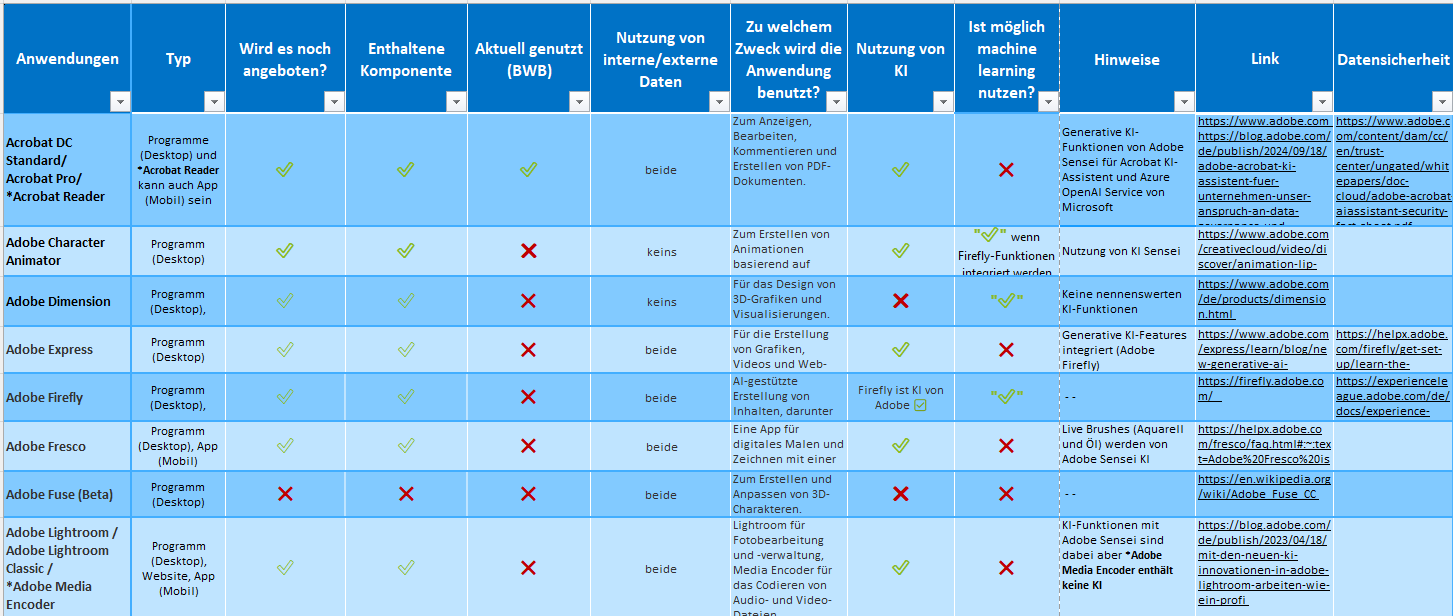
\includegraphics[width=\textheight]{BILDER-PTB2/Adobe.Liste.1.png}
        \end{minipage}
    \end{adjustbox}
\end{center}
\vspace*{\fill}

\vspace*{\fill}
\begin{center}
    \begin{adjustbox}{rotate=90, center, valign=b}
        \begin{minipage}{0.95\textheight}
            \centering
            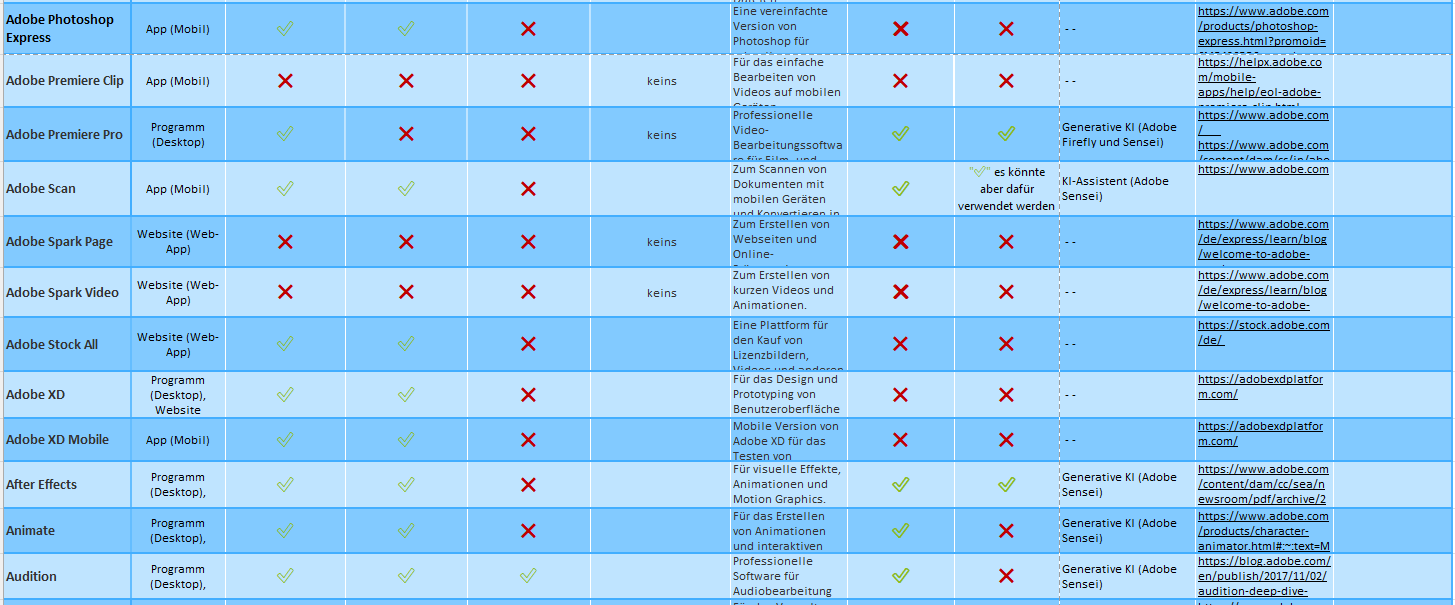
\includegraphics[width=\textheight]{BILDER-PTB2/Adobe.Liste.2.png}
        \end{minipage}
    \end{adjustbox}
\end{center}
\vspace*{\fill}

\vspace*{\fill}
\begin{center}
    \begin{adjustbox}{rotate=90, center, valign=b}
        \begin{minipage}{0.95\textheight}
            \centering
            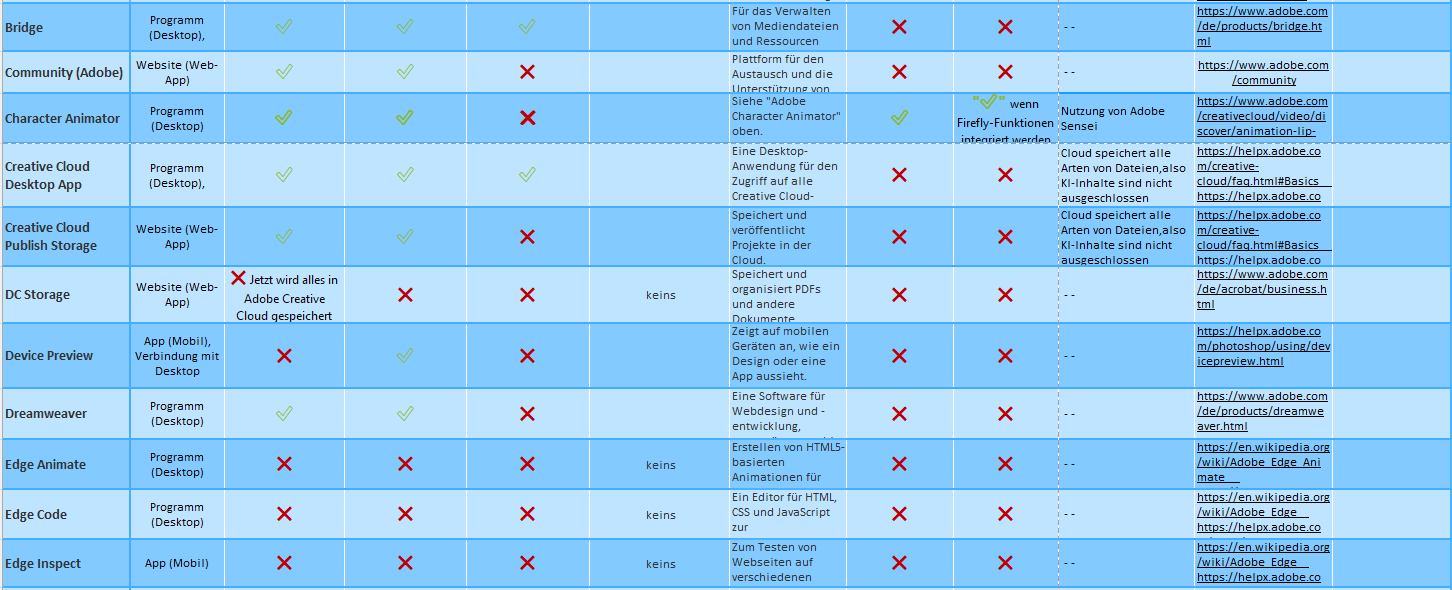
\includegraphics[width=\textheight]{BILDER-PTB2/Adobe.Liste.3.png}
        \end{minipage}
    \end{adjustbox}
\end{center}
\vspace*{\fill}

\vspace*{\fill}
\begin{center}
    \begin{adjustbox}{rotate=90, center, valign=b}
        \begin{minipage}{0.95\textheight}
            \centering
            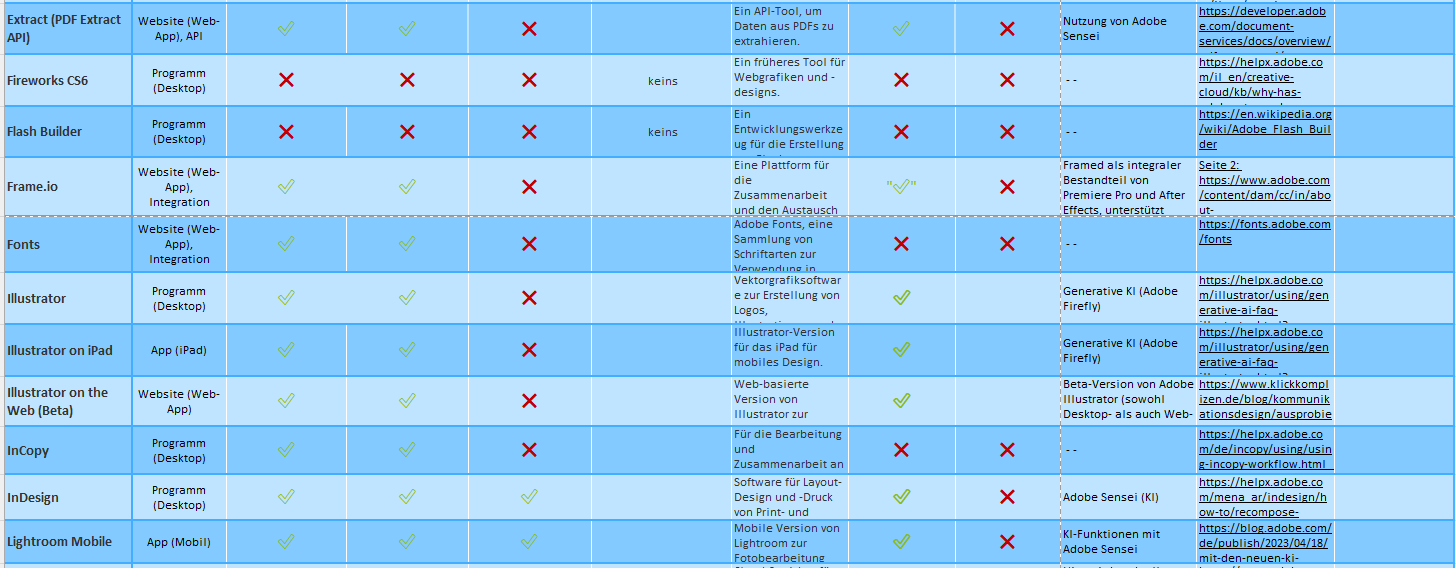
\includegraphics[width=\textheight]{BILDER-PTB2/Adobe.Liste.4.png}
        \end{minipage}
    \end{adjustbox}
\end{center}
\vspace*{\fill}

\vspace*{\fill}
\begin{center}
    \begin{adjustbox}{rotate=90, center, valign=b}
        \begin{minipage}{0.95\textheight}
            \centering
            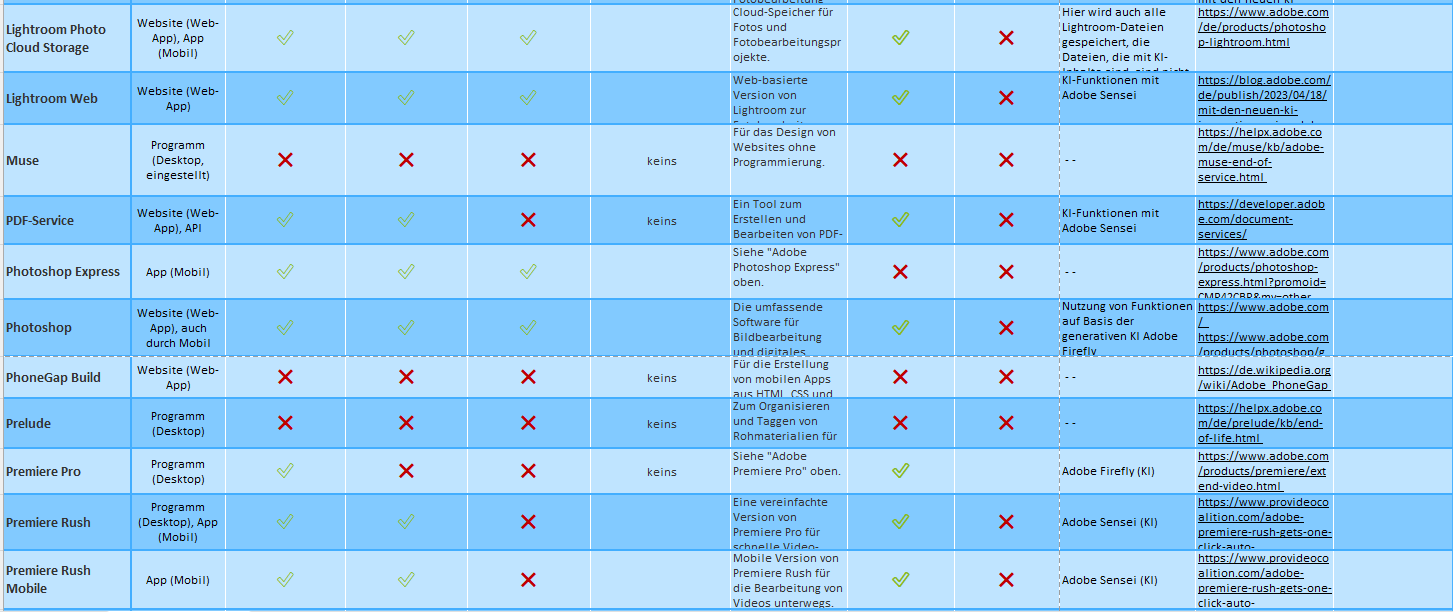
\includegraphics[width=\textheight]{BILDER-PTB2/Adobe.Liste.5.png}
        \end{minipage}
    \end{adjustbox}
\end{center}
\vspace*{\fill} 

% Anhang 2
\newpage
\phantomsection
\addcontentsline{toc}{subsection}{Anhang 2: Interviewprotokoll}
\label{sec:Anhang2}

{\Large\bfseries Anhang 2: Interviewprotokoll}\\[1em]
\textbf{Interviewer:} Nicole Camille Baião \\
\textbf{Befragter:} Pascale Siegel (IT-Portfolio-Managerin) \\
\textbf{Datum:} 01. September 2025 \\
\textbf{Ort:} Berliner Wasserbetriebe, Neue Jüdenstraße 2, 10179 Berlin 
\subsection*{Einstieg ins Thema}

\textbf{Frage 1:} Können Sie sich kurz vorstellen und Ihre Rolle im Portfolio-Management beschreiben?  

Mein Name ist Pascale Siegel, ich bin IT-Portfolio-Managerin bei den Berliner Wasserbetrieben. Das bedeutet, dass ich das IT-Vorhabenportfolio betreue – vom Antrag eines IT-Vorhabens bis zur Übergabe an die Verantwortlichen des Vorhabens (vergleichbar mit Projektleitern), die die Umsetzung übernehmen. Meine Aufgabe ist es, auf übergeordneter Ebene bestimmte Prüf- und Entscheidungsprozesse zu steuern, Genehmigungen oder Ablehnungen in entsprechenden Gremien herbeizuführen, alles zu dokumentieren und den Überblick über alle IT-Projekte zu behalten. Bei Bedarf bereite ich außerdem Auswertungen für wichtige Stakeholder auf.  

\textbf{Frage 2:} Wie kam die Anfrage zur verstärkten Nutzung von KI-gestützter Software (wie der Adobe Creative Cloud) bei Ihnen an, und was waren Ihre ersten Überlegungen dazu?  

Die Anfrage entstand, weil die Unternehmenskommunikation seit Jahren Adobe Creative Suite nutzte, dieses Produkt aber nicht mehr verfügbar ist und durch die Adobe Creative Cloud abgelöst wurde. Um die Arbeitsfähigkeit des Fachbereichs aufrechtzuerhalten, stellten wir daher auf die Creative Cloud um – vorerst allerdings nur in dem Umfang der bisher genutzten Funktionen. Neue Komponenten, insbesondere solche mit KI-Funktionen, blieben zunächst deaktiviert, da deren Einführung einer umfassenden Prüfung bedarf. Unsere ersten Überlegungen gingen somit in zwei Richtungen: Einerseits wollten wir dem Bedarfsträger schnell eine Lösung bieten, andererseits mussten wir das neue Cloud-basierte, KI-gestützte Produkt vor einer vollständigen Freigabe gründlich prüfen. Generell werden bei uns alle neuen Produkte – vor allem Cloud-Dienste – vor der Einführung detailliert überprüft.  

\subsection*{Erste Schritte und Abstimmungen}

\textbf{Frage 3:} Welche Abstimmungen mit anderen Abteilungen wurden am Anfang durchgeführt, und mit wem haben Sie zuerst gesprochen?  

Für neue Produkte gibt es bei uns vordefinierte Abstimmungsrunden. Üblicherweise müssen zunächst Bereiche wie IT-Sicherheit und Datenschutz einbezogen werden. In diesem Fall war die Situation speziell, da der Fachbereich das Vorgängerprodukt bereits einsetzte und wir aus betrieblichen Gründen schnell auf die Cloud umstellen mussten. Einige Abstimmungen haben wir daher im Nachgang durchgeführt. Nichtsdestotrotz wurden die üblichen Stellen einbezogen: Wir haben mit der IT-Sicherheit und dem Datenschutz gesprochen und den Fachbereich (den internen Kunden) darüber informiert, dass keine zusätzlichen Tools freigeschaltet werden, bevor alle Prüfungen abgeschlossen sind. Intern haben wir uns außerdem mit den zuständigen IT-Betreuern abgestimmt; je nach Umfang des Themas würde auch die Arbeitnehmervertretung frühzeitig eingebunden. Kurz gesagt, gibt es einen festen Kreis an Beteiligten, mit denen zu Beginn gesprochen werden muss.  

\textbf{Frage 4:} Gab es dabei von Anfang an besondere Bedenken oder bereits klare Vorgaben seitens bestimmter Stellen?  

Grundsätzlich gibt es eine vorgegebene Vorgehensweise – also klare Vorgaben, welche Stellen involviert werden müssen. Neu und unklar war in diesem Fall allerdings der Umgang mit der KI-Komponente. Für uns war das Thema KI noch Neuland, da eine unternehmensweite KI-Richtlinie zu dem Zeitpunkt erst in Arbeit war. Zu Beginn war daher nicht eindeutig, worauf wir den Fokus legen sollten: auf die KI-Funktion selbst, auf das Tool als Ganzes oder auf die Tatsache, dass es sich um einen Cloud-Dienst handelt. Die Prüfung cloudbasierter Software gehört zwar bereits zum Standardprozedere, aber der Aspekt KI stellte eine neue Herausforderung dar.  

\subsection*{Informationsbedarf}

\textbf{Frage 5:} Welche Methoden zur Bewertung der Software haben Sie in Betracht gezogen und warum haben Sie sich für das Memo und die Excel-Tabelle als Instrumente entschieden?  

Wir haben uns für ein ausführliches Memo und eine Excel-Übersicht entschieden, da sich das Thema als sehr komplex herausgestellt hat. Das Memo diente dazu, allen Beteiligten vorab einen verständlichen Überblick zu verschaffen. Es hilft insbesondere auch Kollegen ohne tiefes IT-Wissen, den Kern des Themas zu erfassen. Die Excel-Tabelle war ein neues Werkzeug, das wir entwickelt haben, um die Adobe Creative Cloud in ihre vielen Einzelkomponenten aufzuschlüsseln. Darin haben wir jede Komponente aufgelistet und vermerkt, ob sie bereits genutzt wird, ob sie KI-gestützt ist und – wenn ja – welche KI-Funktion dahintersteckt. Diese detaillierte Aufstellung war wichtig, um den gesamten Umfang des Produkts zu verstehen und eine fundierte Bewertung durchführen zu können. Im Nachhinein hat sich gezeigt, dass die Tabelle äußerst hilfreich war: Sie verschaffte allen Beteiligten einen klaren Überblick und wurde in den internen Rückmeldungen ausdrücklich gelobt.  

\textbf{Frage 6:} Welche Informationen waren notwendig, um die Anfrage zur Adobe Creative Cloud zu bewerten, und warum waren gerade diese Aspekte entscheidend?  

Entscheidende Informationen betrafen vor allem den Anbieter und die Datenverarbeitung. Wir mussten wissen, wo der Anbieter sitzt bzw. wo die Daten liegen – bei einem europäischen Anbieter bleiben die Daten in Europa, was für uns als kritisches Infrastrukturunternehmen sehr wichtig ist. Außerdem war relevant, welche Art von Daten mit dem Tool verarbeitet würden, also ob es sich um interne, eventuell sensible Daten oder um unkritische/öffentliche Inhalte handelt. Diese Punkte beeinflussen die Risikobewertung maßgeblich: Wenn etwa ein Dienstleister außerhalb der EU agiert oder hochsensible interne Daten verarbeitet würden, wäre das für uns potenziell ein Ausschlusskriterium.  

\subsection*{Bewertung der KI-Funktionen}

\textbf{Frage 7:} Wie hat die KI-Integration in der Adobe Creative Cloud die Bewertung beeinflusst, und welche Risiken und Chancen wurden dabei diskutiert?  

Die Integration von KI-Funktionen hat die Bewertung deutlich beeinflusst. Alle KI-gestützten Features wurden vorerst deaktiviert und dürfen erst genutzt werden, nachdem sämtliche Prüfschritte durchlaufen und eine Freigabe erteilt worden sind. Im Bewertungsprozess mussten wir zusätzlich klären, ob es sich bei den neuen Funktionen um selbstlernende KI handelt und welche Inhalte überhaupt in die Cloud hochgeladen werden dürfen, um dort von der KI verarbeitet zu werden. Als Risiko wurde vor allem diskutiert, dass sensible interne Informationen (z.\,B. detailreiche Bilder unserer Anlagen) keinesfalls ungeschützt in eine KI-Bearbeitung gelangen dürfen, weil solche Daten nicht öffentlich werden dürfen. Entsprechende Inhalte müssten also vor einem Upload für KI-Anwendungen unkenntlich gemacht werden. Auf der Chancen-Seite bieten die KI-Funktionen ein großes Potenzial zur Zeitersparnis: Kreativinhalte – etwa Bilder oder Texte – können deutlich schneller und in größerer Vielfalt erstellt werden, was der Unternehmenskommunikation in ihrer Arbeit zugute käme.  

\textbf{Frage 8:} Wie verlief die Zusammenarbeit mit den beteiligten Abteilungen, und welche Schwierigkeiten traten in der Abstimmung auf?  

Die bereichsübergreifende Zusammenarbeit war anspruchsvoll, weil das Thema so komplex ist. Es waren mindestens zwei Abstimmungsrunden mit den relevanten Abteilungen nötig (etwa mit IT-Sicherheit, Unternehmensstrategie/-entwicklung und Datenschutz). Zunächst musste in einem Vorbereitungsgespräch ein gemeinsames Grundverständnis geschaffen werden, bevor in größerer Runde überhaupt sachgerecht bewertet werden konnte. Im eigentlichen Bewertungstermin haben wir dann ebenfalls Zeit darauf verwendet, sicherzustellen, dass alle Beteiligten das Ziel der Bewertung verstehen. Die Excel-Übersicht erwies sich dabei als sehr hilfreich: wir konnten gemeinsam in der Tabelle nachvollziehen, welche Komponenten der Adobe Cloud betrachtet werden und welche Funktionen (inklusive KI) damit jeweils verbunden sind. Die größte Hürde war letztlich, in kurzer Zeit alle Beteiligten auf denselben Wissensstand zu bringen, um eine fundierte Risikoabschätzung zu ermöglichen.  

\textbf{Frage 9:} Zu welchem Ergebnis ist die Prüfung bisher gekommen? Gab es bereits greifbare Ergebnisse nach der Recherche und den Abstimmungsrunden?  

Ein endgültiges Ergebnis liegt noch nicht vor. Die bisherigen Analysen und Abstimmungen haben aber gezeigt, dass wir die Freigabe der Adobe Creative Cloud sehr differenziert betrachten müssen. Technisch können die KI-basierten Funktionen entweder für alle aktuellen Nutzer freigeschaltet werden oder für niemanden – eine selektive Freigabe pro Fachbereich ist nicht möglich. Bisher darf die Unternehmenskommunikation die Cloud nur in eingeschränktem Umfang nutzen. Unsere Risikoanalyse deutet darauf hin, dass die Unternehmenskommunikation unter ihren vorhandenen Sicherheitsvorgaben wahrscheinlich auch die KI-Funktionen nutzen könnte, da sie größtenteils mit unkritischen, publikationsfähigen Inhalten arbeitet. Für andere Fachbereiche (wie z.\,B. Planung und Bau), die das Tool ebenfalls einsetzen, haben wir die Risiken hingegen noch nicht im Detail bewertet. Es ist also weiterhin unklar, ob die vollständige Nutzung der KI-Komponenten für alle Bereiche unbedenklich möglich wäre.  

\subsection*{Strategische Einordnung}

\textbf{Frage 10:} Welche Rolle spielt das Portfolio-Management bei der Einordnung von KI-gestützten Anwendungen wie Adobe Creative Cloud in die Gesamtstrategie der BWB?  

Bei der strategischen Einordnung solcher KI-gestützten Anwendungen hat das Portfolio-Management selbst wenig Einfluss. Im Unternehmen wurde hierfür eine bereichsübergreifende Expertengruppe ins Leben gerufen, die eine KI-Policy ausarbeitet und das Thema umfassend beleuchtet. Diese Expertengruppe wird die Leitlinien für den Umgang mit KI erarbeiten und in die Unternehmensstrategie einfließen lassen. Das Portfolio-Management ist in diese strategische Arbeitsgruppe nicht direkt eingebunden und konzentriert sich eher auf die operative Ebene – also darauf, einzelne Vorhaben zu prüfen und umzusetzen, anstatt strategische KI-Grundsätze festzulegen.  

\textbf{Frage 11:} Gibt es definierte Kriterien oder Standards, nach denen entschieden wird, ob eine Software eingeführt oder abgelehnt wird?  

Ja, wir verfügen über einen klar definierten Prozess für solche Entscheidungen. Bevor eine Software eingeführt werden kann, muss der Bedarf vom anfordernden Fachbereich formell gestellt werden – in unserem Fall durch einen Antrag im IT-Serviceportal. Dieser Antrag (für neue oder zu ändernde Software, Hardware oder Dienstleistungen) wird nacheinander von verschiedenen Stellen geprüft, darunter z.\,B. das IT-Architekturmanagement, das Portfolio-Management, das Bestands- und das Change Management. Jede dieser Instanzen bewertet den Antrag aus ihrer Perspektive. Anschließend wird der Antrag in einem IT-Gremium vorgelegt, das gemeinsam entscheidet, ob die Einführung des Produkts grundsätzlich machbar und sinnvoll ist. Dabei wird beispielsweise betrachtet, ob bereits ein vergleichbares Produkt im Haus existiert oder ob bestimmte Risiken gegen die Einführung sprechen. Wenn das Gremium grünes Licht gibt und alle weiteren entscheidungsbefugten Stellen (bis hin zur IT-Leitung) zugestimmt haben, geht das Vorhaben in die Beschaffung. Als öffentliches Unternehmen unterliegen wir in der Beschaffung strengen Vorgaben (z.\,B. Ausschreibungspflichten), die ebenfalls eingehalten werden müssen, bevor eine Software letztlich zum Einsatz kommen kann.  

\subsection*{Ausblick}

\textbf{Frage 12:} Gibt es bereits eine finale Entscheidung in dieser Angelegenheit? Wenn nicht, welche möglichen Lösungen sehen Sie, und welche nächsten Schritte sind geplant?  

Eine endgültige Entscheidung steht noch aus, und derzeit werden verschiedene Lösungsszenarien geprüft. Entweder führen wir für jeden betroffenen Fachbereich eine separate Risikobewertung durch und könnten bei durchweg positiven Ergebnissen die KI-Funktionen für alle freigeben – oder wir erlauben die volle Nutzung nur der Unternehmenskommunikation und belassen die übrigen Fachbereiche bei der bisherigen eingeschränkten Nutzung. In letzterem Fall müsste man für die anderen Bereiche gegebenenfalls Alternativlösungen ohne KI-Funktionalität finden. Diese Optionen werden derzeit intern abgewogen. Die nächsten Schritte sind, die noch ausstehenden Prüfungen durchzuführen (insbesondere die Risikobetrachtung für weitere interessierte Fachbereiche) und die Ergebnisse mit der in Entwicklung befindlichen KI-Policy des Unternehmens abzugleichen. Erst auf dieser Grundlage wird eine finale Entscheidung getroffen.  

\textbf{Frage 13:} Gibt es eine bevorzugte Vorgehensweise – etwa zunächst Alternativen prüfen, auf KI-Freigaben warten oder vorerst eine Software ohne KI nutzen?  

Derzeit gibt es keine eindeutige Präferenz. Vorrangig sollen zunächst alle laufenden Prüfungen und Abstimmungen abgeschlossen werden – insbesondere die noch ausstehenden Risikobewertungen für andere Fachbereiche sowie die Fertigstellung der internen KI-Richtlinie. Auf dieser Basis wird dann entschieden, wie wir weiter vorgehen. Bis dahin gilt es, umsichtig zu bleiben: Wir halten an der eingeschränkten Nutzung fest, bis klare interne Vorgaben zur KI-Nutzung vorliegen. Parallel behalten wir mögliche alternative Lösungen im Blick, doch zunächst warten wir die Ergebnisse der laufenden Prüfungen ab.



% === Ehrenwörtliche Erklärung ===
\newpage
\section*{Ehrenwörtliche Erklärung}
\addcontentsline{toc}{section}{Ehrenwörtliche Erklärung}

„Ich erkläre ehrenwörtlich:

\begin{itemize}
    \raggedright
    \item \normalsize dass ich meinen Praxistransferbericht ohne fremde Hilfe erstellt habe,
    \item \normalsize dass ich wörtliche Zitate aus der Literatur – etwa aus Büchern, wissenschaftlichen Artikeln oder offiziellen Quellen – entnommen und entsprechend gekennzeichnet habe,
    \item \normalsize dass ich Künstliche Intelligenz zur Formulierung einiger Sätze verwendet habe, und ebenfalls zur Korrektur der grammatikalischen Fehler beim Schreiben“
\end{itemize}
„Alle Quellen, die aus dem Internet oder aus anderen digitalen Medien stammen, die für den Praxistransferbericht verwendet wurden, sind der Arbeit beigefügt.“

„Ich bin mir bewusst, dass eine falsche Erklärung rechtliche Konsequenzen nach sich zieht“.\\

% --- Tabelle mit Unterschriften ---

\begin{tabular}{p{8cm}}
    \normalsize{Berlin, den XX. XXXX 202X} \\[0.5cm]
    
\includegraphics[width=5.5cm]{BILDER-PTB2/unterschrift_nicole.png} \\
    \normalsize{\underline{\hspace{5.5cm}}} \\
    \normalsize{(Unterschrift der Studentin)}
\end{tabular} % \underline{\hspace{6cm}} erzeugt eine Linie mit einer Länge von 6 cm


% === ENDE DOKUMENT ===
\end{document}